\section{System Overview}

Though it may appear trivial at first, the broad scope of the design space of this project meant making difficult design decisions where there was often no clear answer.  The first major decision was determining the approach used to reduce the swapping time.  Inspired by the battery connectors in some wearable devices, a hot swapping connector design was chosen.  Hot swapping refers to the ability to connect or disconnect a peripheral, in this case a guitar pedal, without needing to perform any special preparatory actions such as turning off the power.  This type of design unites a physical action of inserting or removing a pedal into a system with the electrical switching actions required to actually perform the hot swapping.

With this decision made, the high level design of the hot swapping device was considered.  To be able to insert a pedal into the signal chain at any time meant that the solution required a main signal control device, which acts as a "meta pedal", connected between the guitar and an amplifier.  When the hot swapping device is not activated, the guitar signal is connected directly to the amplifier.  When the hot swapping action occurs, the signal is routed through the hot swapping connector to the pedal and back, allowing the pedal to be inserted into the signal chain between the guitar and amplifier.

This required standardizing the interface between the guitar pedal and the device.  Data collected during a site visit to a Guitar Center retail location demonstrated the plethora of effects pedals available at a standard brick-and-mortar store.  These 150 pedals represent a good mix of products, from mass market production units such as the Boss DS-1 to high quality and expensive effects like Eventide’s H9. While the major manufacturers like Boss, MXR, and Electro Harmonix have narrowed their form factors down to a handful of types each, there is no standardization across producers on features important for this project, including the dimensions of the enclosure, the location and orientation of the signal and power jacks, the location of the screws used to hold the pedal’s bottom plates. Though most products use the de facto standard 9 VDC, center negative power supply connected with a 2.1 mm plug, this too has variations in some cases. All of these variations complicate standardizing a form that can easily be hot swapped.  A universal adapter was designed to connect the pedal to the hot swapping device.

On a high level, the design process focused on ease of use and intuition for the user over any other considerations where possible, which explains the preference for this tactile and tangible hot swapping method over a programmable switching device, for instance.  The push for simplicity has led to some increases in design complexity, including the need to automatically detect when a hot swapping event occurs rather than include a separate user controlled switch.

In order for a user to be able to test multiple effects, multiple hot swapping devices were included in the device.  An internal signal routing system was also designed to facilitate testing pedals in different routing configurations including series, parallel, feedback, and various combinations of these.  Finally, a user interface was designed to control this internal signal routing.

Because of the repetition present in the device, it was designed as a modular system to simplify design, fabrication, and evaluation.  Figures \ref{fig:system_block} and \ref{fig:module_block} show a hierarchical block diagram of the system.  The system level diagram shows three modules were used for the full implementation of the system, with only audio passing between them.  The same $24VDC$ power input was passed to each module.  The module level diagram shows the major constituent parts of each module.  The design and function of each of these will be discussed in the remainder of this chapter.

\insertimage{0.95}{FinalImages/SystemBlock_white.jpg}{System level of hierarchical block diagram.  This shows the modular design of the device.  The legend in the upper right shows that power is indicated in red, audio signal in black, and control signals in green, with the direction of the arrow indicating data direction.  Note that no control signals pass between the modules, making design and debugging simple.  The signal and power I/O for the device are passed on to the modules.}{fig:system_block}

\insertimage{0.95}{FinalImages/ModuleBlock_white.jpg}{Module level block diagram showing the contents of each module.  As in Figure \ref{fig:system_block}, power is indicated in red, audio signal in black, and control signals in green, with the direction of the arrow indicating data direction.  In principle, each module contains a pair of hot swap devices consisting of the hot swap connector, DPDT switching element, and adjustable voltage regulator.  The module also contains an internal signal routing mechanism consisting of two mixers and a user interface, as well as all necessary voltage regulators required to step down the 24V input for all these circuits.}{fig:module_block}

\section{Design Decisions}
	\subsection{Universal Adapter}

	Because of the large variety of guitar pedal shapes, they are not by themselves suitable for hot swapping in and out of a fixed receiving unit. A universal adapter was designed to interface between the pedal's I/O and the hot swapping connector.  The required attributes for this adapter include a way to mechanically mount a pedal, a way to connect to the pedal's I/O, and a way to connect to the hot swapping connector.  The last requirement means that there must be exposed electrodes with which the corresponding electrodes on the main device can make electrical connection.  It also includes a method to physically align these electrodes when the hot swap device is active.  None of these requirement suggest a need for much vertical height, so this universal adapter will in general come in the form a base plate on which the pedal sits.  Because of this, "plate" is used to refer to this universal adapter throughout the rest of this document.  

		\subsubsection{Pedal-Plate Mounting}

		The thin and flat nature of the universal adapter plate allows the plate itself to be used as part of fastening the pedal.  Holes and slots cut into the plate which allow screws to pass open up several options for mounting a pedal.  Because of its simplicity, the most attractive option was to reuse the screws that hold in the pedal's bottom cover.  As most pedal enclosures have bottom covers held on by four screws, one in each corner, reusing two screws in opposite corners to pass through the plate allows the cover to remain in place while still resulting in a good mechanical connection between the pedal and the plate.  However, because a non-trivial number of effects pedal enclosures have fewer bottom plate screws, or none at all, this method is not completely universal.

		To accommodate pedals that do not have the common four-screw bottom plate, a clamping mechanism can be used to modify the method described above.  Instead of reusing pedal's bottom plate screws, a clamp in the shape of a corner bracket is placed over the top corner of the pedal, and a screw is again passed through the plate used to tighten the corner clamp down, securing the pedal along with it.  This solution allows the same type of holes and slots used with the direct bottom cover screw method.  The clamp should be padded to prevent damage to the product.  Although this augmentation to the bottom cover screw method would help to increase compatibility, it was not explored further due to time constraints.

		The advantage of both of these methods is that they are easily reversible and have no lasting effects on the appearance or function of the product.  However, if neither of the above attachment methods was adequate, velcro could also be used to attach the pedal to the plate, as is common with permanent pedalboard setups.  However, this can leave a residue on the product so it is less desirable.

		\Huge INSERT IMAGE OF CORNER BRACKET clamp \\
		\normalsize

		\subsubsection{Plate Size}

		The position and dimension of the slots and holes required for the through-screw methods of mechanical attachment mentioned above must be positioned to allow alignment with the pedal's bottom cover screw holes.  Because this varies with the exact geometry of the enclosure, these holes should allow for adjustment.  Slots were chosen over holes as the primary mating location because of their allowance for adjustment along an axis.  To determine the exact shape of the slots, measurements of the physical dimensions of pedals at Guitar Center were taken, to determine a guideline to estimate the relative position of the bottom plate screw holes compared to the outer dimensions of the enclosure.  Based on the measurements taken, the distance between screws in any direction is typically 90\% to 95\% of the outer length of the enclosure in that dimension.  Using this, the physical outer dimensions of all of the pedals cataloged at Guitar Center were recorded from each pedal's user manual.

		Because only two screws located on opposite corners of the pedal are used to attach the pedal to the plate, a line can always be draw through both of them\footnote{This is very trivial}.  Therefore, when designing the mounting slots on the plate it is sufficient only to consider the length of this line segment connecting the two screw locations.  Variations in the aspect ratio of the enclosure (width to height) can be dealt with via small rotations.  The data collected from Guitar Center stock was used to actually design the minimum and maximum screw-hole-distances that must be covered.

		First, the data was broken down by company, and each company was assigned a numerical ID.  The number of pedals available from each manufacturer was counted.  Then the data was further broken down by pedal enclosure category.  Generally, each manufacturer will design many of their products to fit in the same enclosure, which keeps their procurement and design process simpler.  This allows the pedals to be grouped by enclosure type, meaning that all pedals offered with the same enclosure will have the same external dimensions and be mechanically compatible with the hot swapping device if any one of them is compatible.  Each enclosure type was also given an ID number, and was labeled with the company who uses it and the number of products being offered by that company using this enclosure type.  This data was plotted using a stacked bar graph as seen in Figure \ref{fig:pedalsAvailable}, with the company ID numbers listed in Table \ref{tab:pedal_companies}.  Note for instance that Company 12 (Boss) offers more than thirty pedals, and the vast majority of these use the same variety use the same type of enclosure, meaning that compatibility with this type of enclosure is a greater priority than a lesser used one, such as the type used by Company 9 (ProCo).  Note also that the plot only shows effects with their physical dimensions listed in the manual, which explains why J Rockett Audio, which had two products, has no bar on the graph.

		\begin{figure}
			\centering
			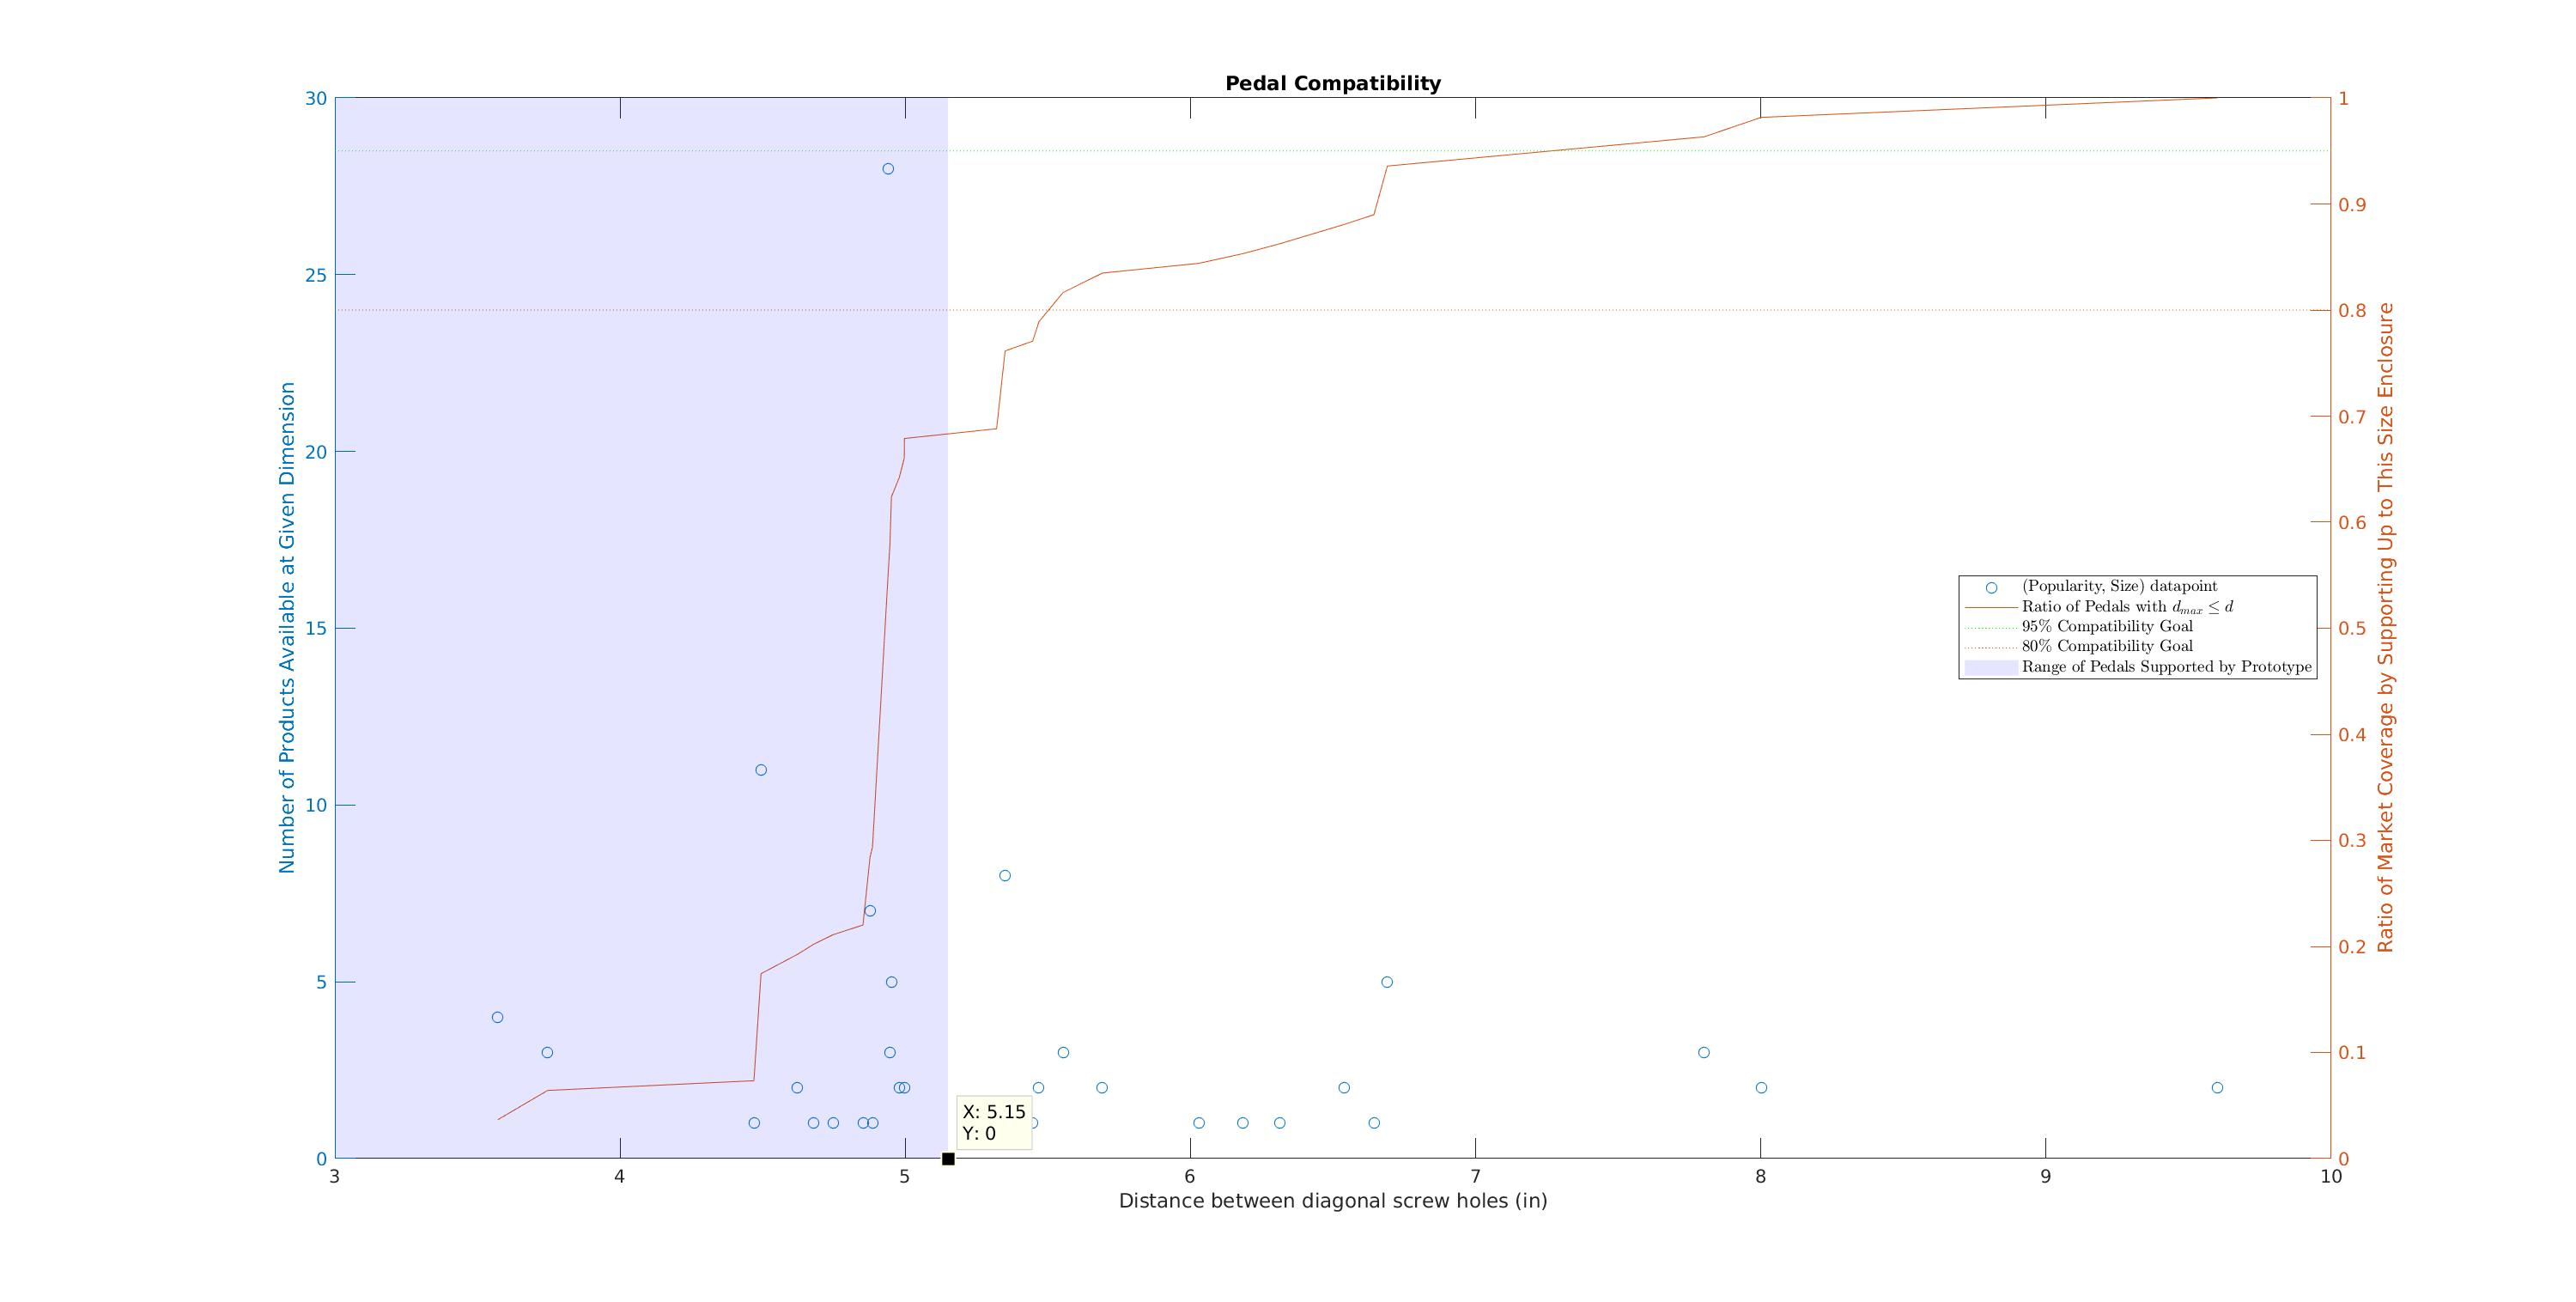
\includegraphics[width = 0.8\textwidth]{PR4Images/PedalsAvailable.jpg}
			\caption{Number of guitar pedals available by manufacturer ID.  The bars are divided vertically by the type of enclosure used, with the most popular enclosures on the bottom.}
			\label{fig:pedalsAvailable}
		\end{figure}


		\begin{table}
		\begin{center}
		\begin{tabular}{ |c c c| }
		\hline
		 Company Name & Company ID & Number of Products Available \\ 
		 \hline
		Seymour Duncan    &  1        &  4     \\
	    BBE               &  2        &  1     \\
	    J Rockett Audio   &  3        &  2     \\
	    Tech 21           &  4        &  2     \\
	    Ampeg             &  5        &  2     \\
	    MXR               &  6        & 18     \\
	    Korg              &  7        &  1     \\
	    Fulltone          &  8        &  6     \\
	    ProCo             &  9        &  1     \\
	    Danelectro        & 10        &  3     \\
	    Digitech          & 11        &  7     \\
	    Boss              & 12        & 33     \\
	    Eventide          & 13        &  1     \\
	    Way Huge          & 14        &  2     \\
	    Egnater           & 15        &  1     \\
	    Line6             & 16        &  1     \\
	    Fender            & 17        &  3     \\
	    Voodoo Lab        & 18        &  1     \\
	    EHX               & 19        & 26     \\
	    Ibanez            & 20        &  5	   \\    
	    Maxon             & 21        &  1     \\
	    EarthQuaker       & 22        &  8     \\
	    JHS               & 23        &  4     \\
	    Keeley            & 24        &  5     \\
	    TC Electronic     & 25        & 13     \\
	   	\hline
		\end{tabular}
		\caption{List of guitar effects manufacturers and their associated ID numbers.}
		\label{tab:pedal_companies}
		\end{center}
		\end{table}

		\insertimage{0.8}{FinalImages/PedalCompatibilityPlot}{Percent of pedals available at a typical retail store that are compatible with plate with diagonal distance $d$.  Because most manufacturers reuse their enclosures for multiple products, it was possible to plot the number of products available in the same enclosure with the diagonal screw distance for that enclosure.  A cumulative ratio of the number of pedals available with this dimension or less was superimposed over these data points.  Because supporting arbitrarily small pedals is not difficult with the design (one long slot would do the job), the plot was used to determine the maximum size slots required to meet the compatibility requirement.  The final design supports a diagonal distance of about 6.5".  The area of the plot less than this dimension was shaded to indicate the pedals supported by the design.  Because the edge of this shaded region intersects the cumulative graph above the green horizontal compatibility goal reference line, this indicates that the design meets this requirement.}{fig:pedalcompatibility}





		\subsubsection{Plate Material}
	\subsection{Hot Swapping Device}
		\subsubsection{Electrical Connection Mechanism}
		\subsubsection{Pedal Power Selection}
		\subsubsection{Hot Swap Event Detection}
		\subsubsection{Hot Swap Event Actuation}
	\subsection{Analog Signal Routing}
		\subsubsection{Routing Architecture}
		\subsubsection{Analog Voltage Supply}
	\subsection{User Interface}
